\documentclass[a4paper]{article}     
\usepackage{amsfonts}
\usepackage{amsmath}
\usepackage{amssymb}
\usepackage{graphicx}
\newcommand{\dint}{\displaystyle\int}

\begin{document}

\noindent \large Auteur: Michaël Francken \\
\noindent \large Studierichting: Informatica\\
\noindent \large Oefeningenreeks 5D nr. 1.12\\

\medskip

\normalsize

$x\sqrt{1-x^2}$ op het interval $[-1,1]$\\

$=x\left(1-x\right)$\\

$=x-x^2$\\

$\displaystyle\int^1_2\left(x-x^2\right)$\\

$=\left[\dfrac{x^2}{2}-\dfrac{x^3}{3}\right]^1_{-1}$\\

$=\left(\dfrac{1^2}{2}-\dfrac{1^3}{3}\right)-\left(\dfrac{\left(-1\right)^2}{2}-\dfrac{\left(-1\right)^3}{3}\right)$\\

$=\dfrac{1}{6}-\dfrac{5}{6}=\dfrac{2}{3}$\\

\begin{figure}[h]
\centering
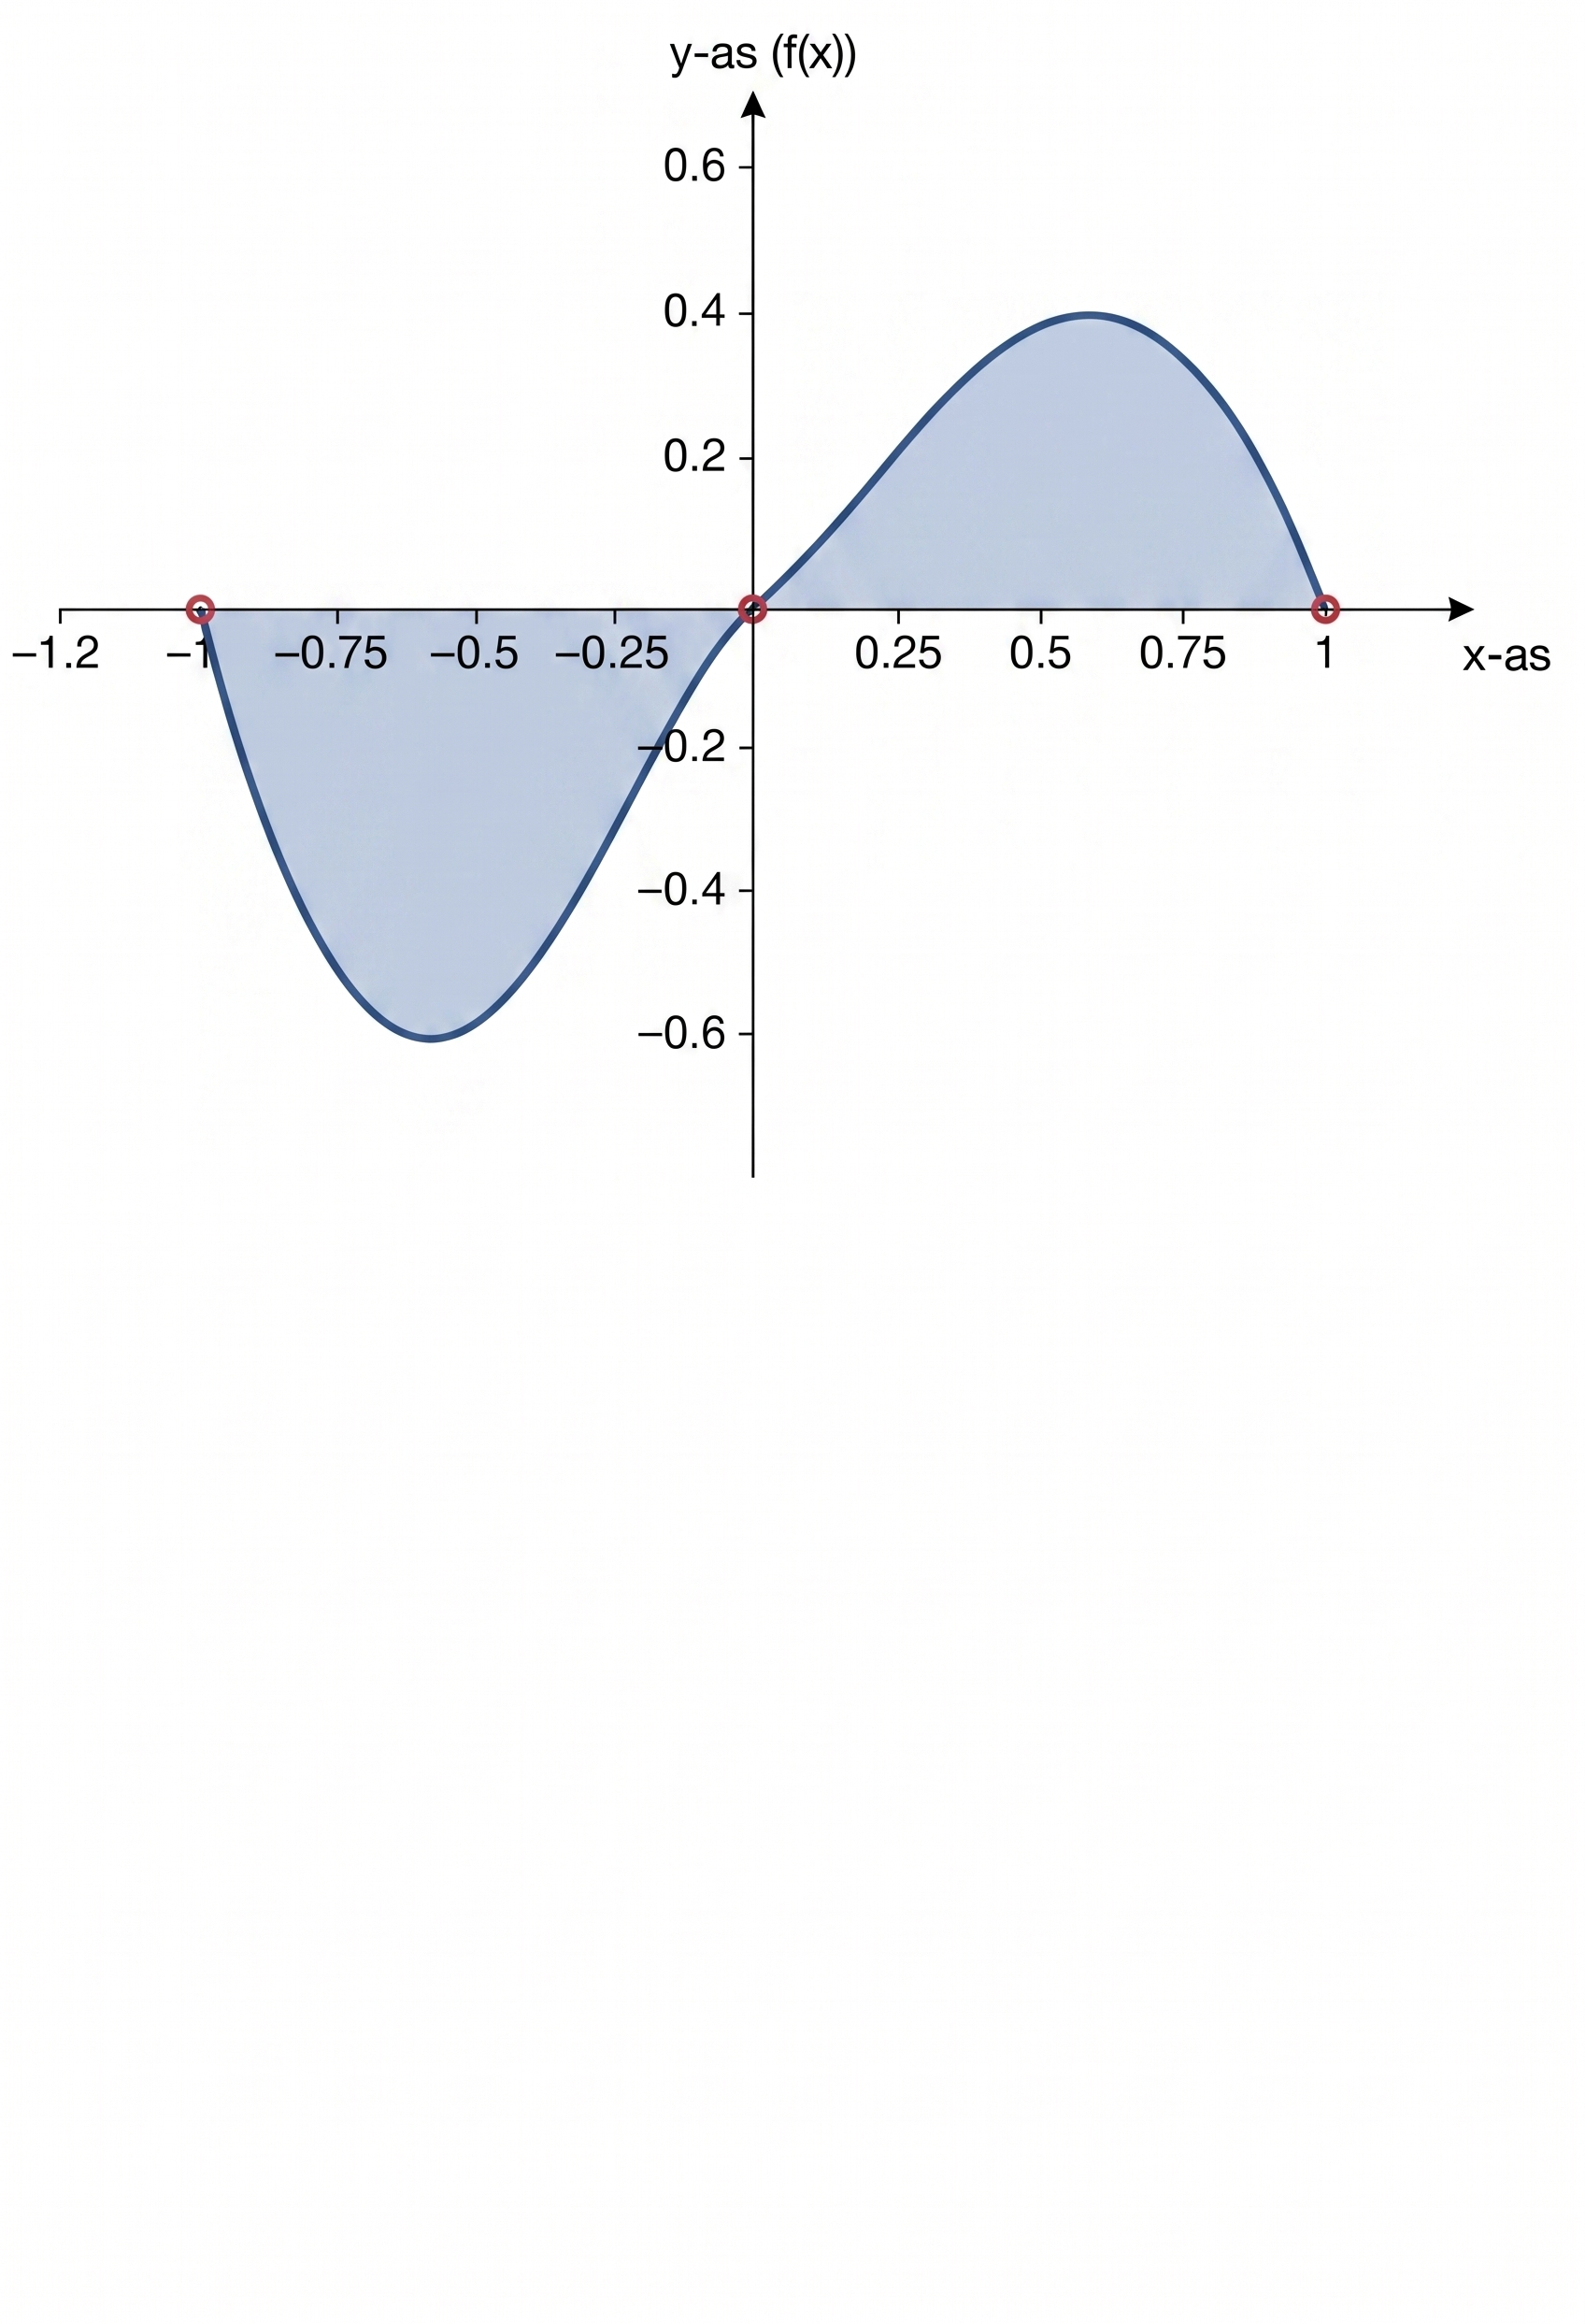
\includegraphics[width=8cm]{5D-1.12-michael.francken.INF.png}
\end{figure}



\begin{thebibliography}{999}
%\bibitem{a} Referentie
\end{thebibliography}
\end{document} 
